\documentclass{beamer}

\usepackage[utf8x]{inputenc}
\usepackage{graphicx}
\usepackage{amsthm,amssymb,amsbsy,amsmath,amsfonts,amssymb,amscd}
\usepackage{dsfont}
\usepackage{array}
\newcolumntype{N}{@{}m{2pt}@{}}
\useoutertheme[subsection=false]{miniframes}
\usepackage{lmodern}

\setbeamercolor{author in head/foot}{fg=gray,bg=white}
\setbeamercolor{title in head/foot}{fg=gray,bg=white}
\setbeamercolor{page number in head/foot}{fg=gray,bg=white}
\setbeamercolor{section in head/foot}{bg=black,fg=gray}
\setbeamercolor{subsection in head/foot}{bg=black,fg=gray}

%%%%%%%%%%%%%%%%%%%%%%%%
% GENERAL BEAMER STYLE :

\setbeamertemplate{footline}{
  \hbox{%
    \begin{beamercolorbox}[wd=.2\paperwidth,ht=2ex,dp=1ex,left]{author in head/foot}%
      \hskip1em\usebeamerfont{author in head/foot}\insertshortauthor
    \end{beamercolorbox}%
    \begin{beamercolorbox}[wd=.7\paperwidth,ht=2ex,dp=1ex,center]{title in head/foot}%
      \usebeamerfont{title in head/foot}\insertshorttitle
    \end{beamercolorbox}%
    \begin{beamercolorbox}[wd=.1\paperwidth,ht=2ex,dp=1ex,right]{page number in head/foot}%
      \usebeamerfont{page number in head/foot}\insertframenumber{} / \inserttotalframenumber
      \kern1em 
    \end{beamercolorbox}
  }
}

\setbeamercolor{alerted text}{fg=red!80!black}
\setbeamercolor{itemize/enumerate subbody}{fg=gray!70!black}
\setbeamertemplate{itemize item}[square]
\setbeamertemplate{itemize subitem}[triangle]%{{\textendash}}
\setbeamerfont{itemize/enumerate subbody}{size=\footnotesize}
\setbeamerfont{itemize/enumerate subitem}{size=\footnotesize}

\setbeamertemplate{navigation symbols}{}

\AtBeginSection{
\begin{frame}
    \begin{centering}
    \begin{beamercolorbox}[sep=12pt,center]{part title}
    \usebeamerfont{section title}\insertsection\par
    \end{beamercolorbox}
    \end{centering}
\end{frame}
}

 

%\title[Short course on Statistical Modelling for Optimization -- lecture 1/4]{ \small Short course Statistical Modelling for Optimization -- lecture 1/4 \\ \vspace{3mm} \LARGE Statistical models in engineering}
%\institute[Mines St-\'Etienne]{Nicolas Durrande (durrande@emse.fr) \\ Jean-Charles Croix (jean-charles.croix@emse.fr) \\ Mines St-\'Etienne -- France}
%\author[Pereira, June 2017]{June 2017 -- Universidad Tecnol\'ogica de Pereira -- Colombia}
\title[\'Ecole chercheurs MEXICO]{ \small \'Ecole chercheurs MEXICO, La Rochelle, Mars 2018\\ \vspace{3mm} \LARGE Introduction to statistical modelling}
\author[\quad La Rochelle, March 2018]{Nicolas Durrande, nicolas@prowler.io}
\institute[]{PROWLER.io, Cambridge (UK) -- Mines St-\'Etienne (France)}
\date{\null}

\DeclareMathOperator*{\Var}{var}
\DeclareMathOperator*{\E}{E}
\DeclareMathOperator*{\Cov}{cov}
\newcommand\PR[1]{\mathrm{P}\left(#1 \right)}
\newcommand\PS[1]{{\langle #1 \rangle}_\mathcal{H}}
\newcommand\PSi[2]{{ \left \langle #1 \right \rangle}_{\! #2}}
\newcommand\N[1]{{|| #1 ||}_\mathcal{H}}
\newcommand\Ni[2]{{|| #1 ||}_{\! #2}}
\newcommand\dx{\, \mathrm{d}}
\newcommand\textequal{\rule[.4ex]{4pt}{0.4pt}\llap{\rule[.7ex]{4pt}{0.4pt}}}
\newcommand{\argmin}{\operatornamewithlimits{argmin}}
\makeatletter
\newcommand{\shorteq}{%
  \settowidth{\@tempdima}{a}% Width of hyphen
  \resizebox{\@tempdima}{\height}{=}%
}
\makeatother

%%%%%%%%%%%%%%%%%%%%%%%%%%%%%%%%%%%%%%%%%%%%%%%%%%%%%%
%%%%%%%%%%%%%%%%%%%%%%%%%%%%%%%%%%%%%%%%%%%%%%%%%%%%%%
%%%%%%%%%%%%%%%%%%%%%%%%%%%%%%%%%%%%%%%%%%%%%%%%%%%%%%
\begin{document}

%%%%%%%%%%%%%%%%%%%%%%%%%%%%%%%%%%%%%%%%%%%%%%%%%%%%%%
\begin{frame}
  \titlepage
\end{frame}

%%%%%%%%%%%%%%%%%%%%%%%%%%%%%%%%%%%%%%%%%%%%%%%%%%%%%%
\begin{frame}{}
Outline of today's lecture
\vspace{0.2cm}
\begin{itemize}
	\item Introduction to costly to evaluate functions.
    \item A few words on statistical modelling.
	\item Design of experiments
\end{itemize}
\end{frame}

%%%%%%%%%%%%%%%%%%%%%%%%%%%%%%%%%%%%%%%%%%%%%%%%%%%%%%
%%%%%%%%%%%%%%%%%%%%%%%%%%%%%%%%%%%%%%%%%%%%%%%%%%%%%%
\section[Context]{Why are statistical models relevant in engineering?}
\subsection{}

%%%%%%%%%%%%%%%%%%%%%%%%%%%%%%%%%%%%%%%%%%%%%%%%%%%%%%
\begin{frame}{}
There is a wide variety of situations where getting data about a system performance can be extremely expensive.
\begin{itemize}
	\item real world experiments
	\item destructive tests
	\item prototyping
	\item numerical experiments
\end{itemize}
\end{frame}

%%%%%%%%%%%%%%%%%%%%%%%%%%%%%%%%%%%%%%%%%%%%%%%%%%%%%%
\begin{frame}{}
\begin{exampleblock}{Example: real world experiments}
\begin{center}
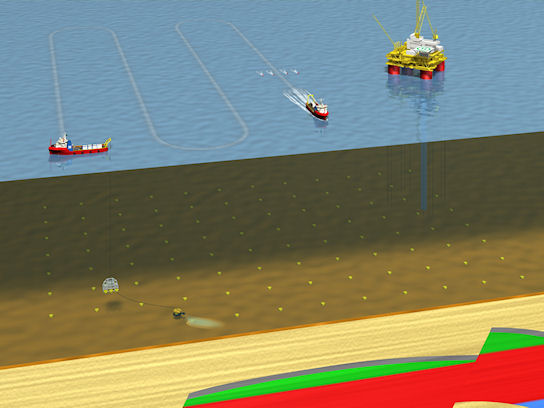
\includegraphics[height=5cm]{figures/drilling}
\end{center}
\end{exampleblock}
\end{frame}

%%%%%%%%%%%%%%%%%%%%%%%%%%%%%%%%%%%%%%%%%%%%%%%%%%%%%%
\begin{frame}{}
\begin{exampleblock}{Example: Destructive tests}
\begin{center}
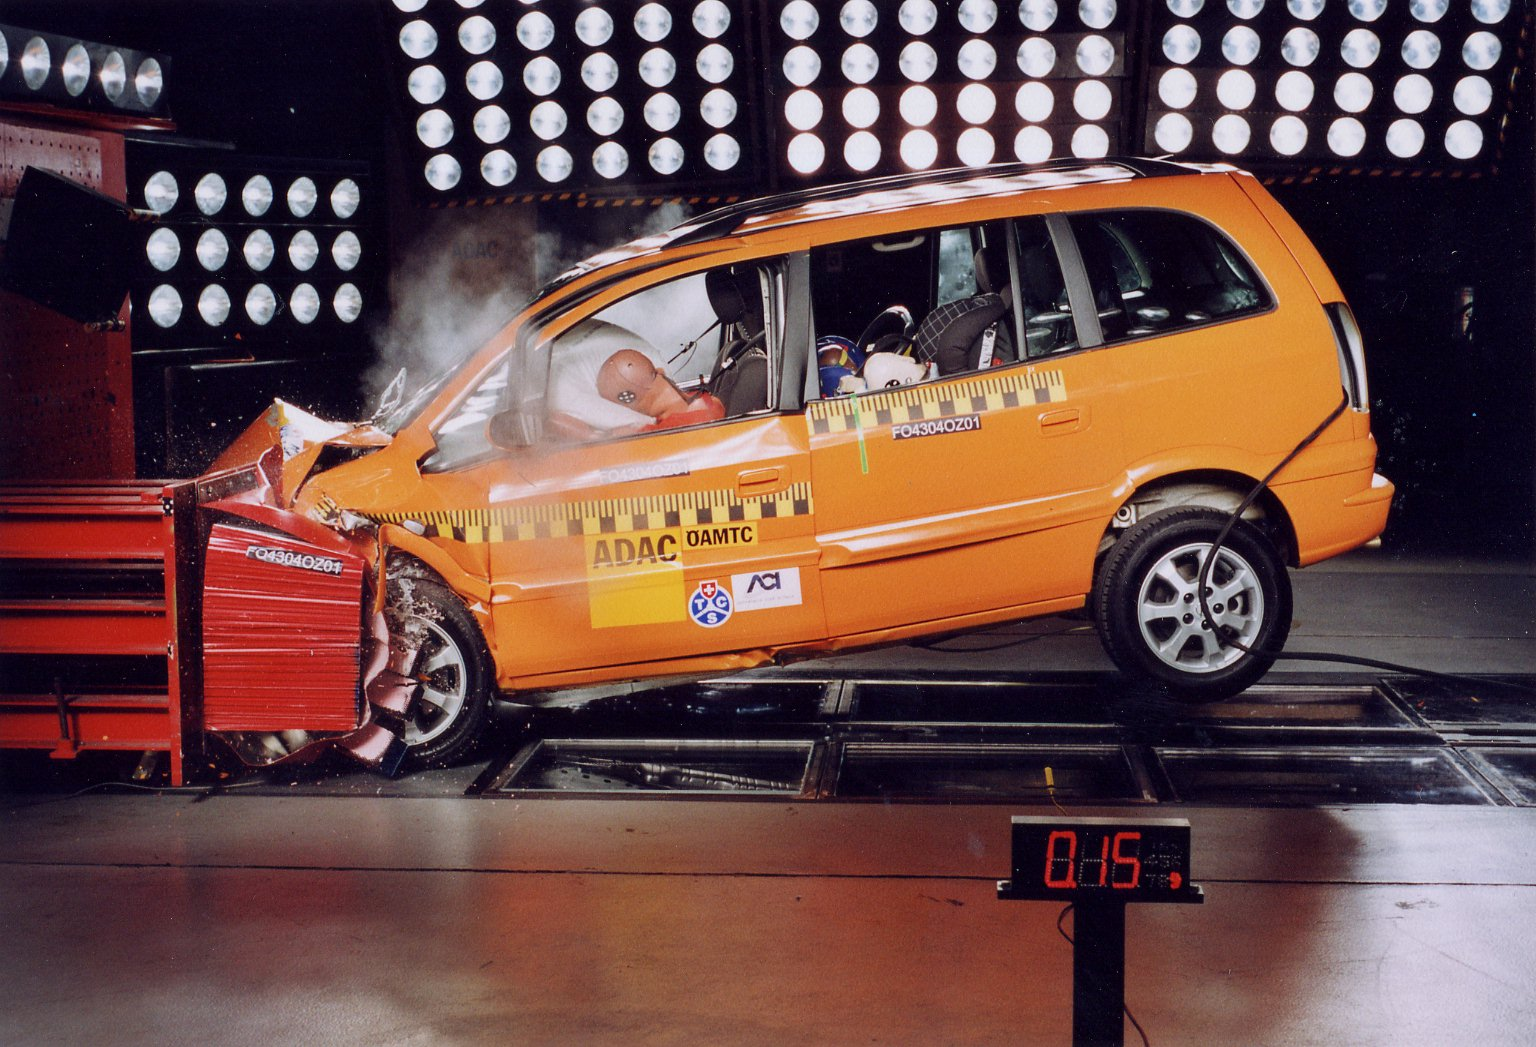
\includegraphics[height=5cm]{figures/crash-test}
\end{center}
\end{exampleblock}
\end{frame}

%%%%%%%%%%%%%%%%%%%%%%%%%%%%%%%%%%%%%%%%%%%%%%%%%%%%%%
\begin{frame}{}
\begin{exampleblock}{Example: Prototyping of a boat shape}
\begin{center}
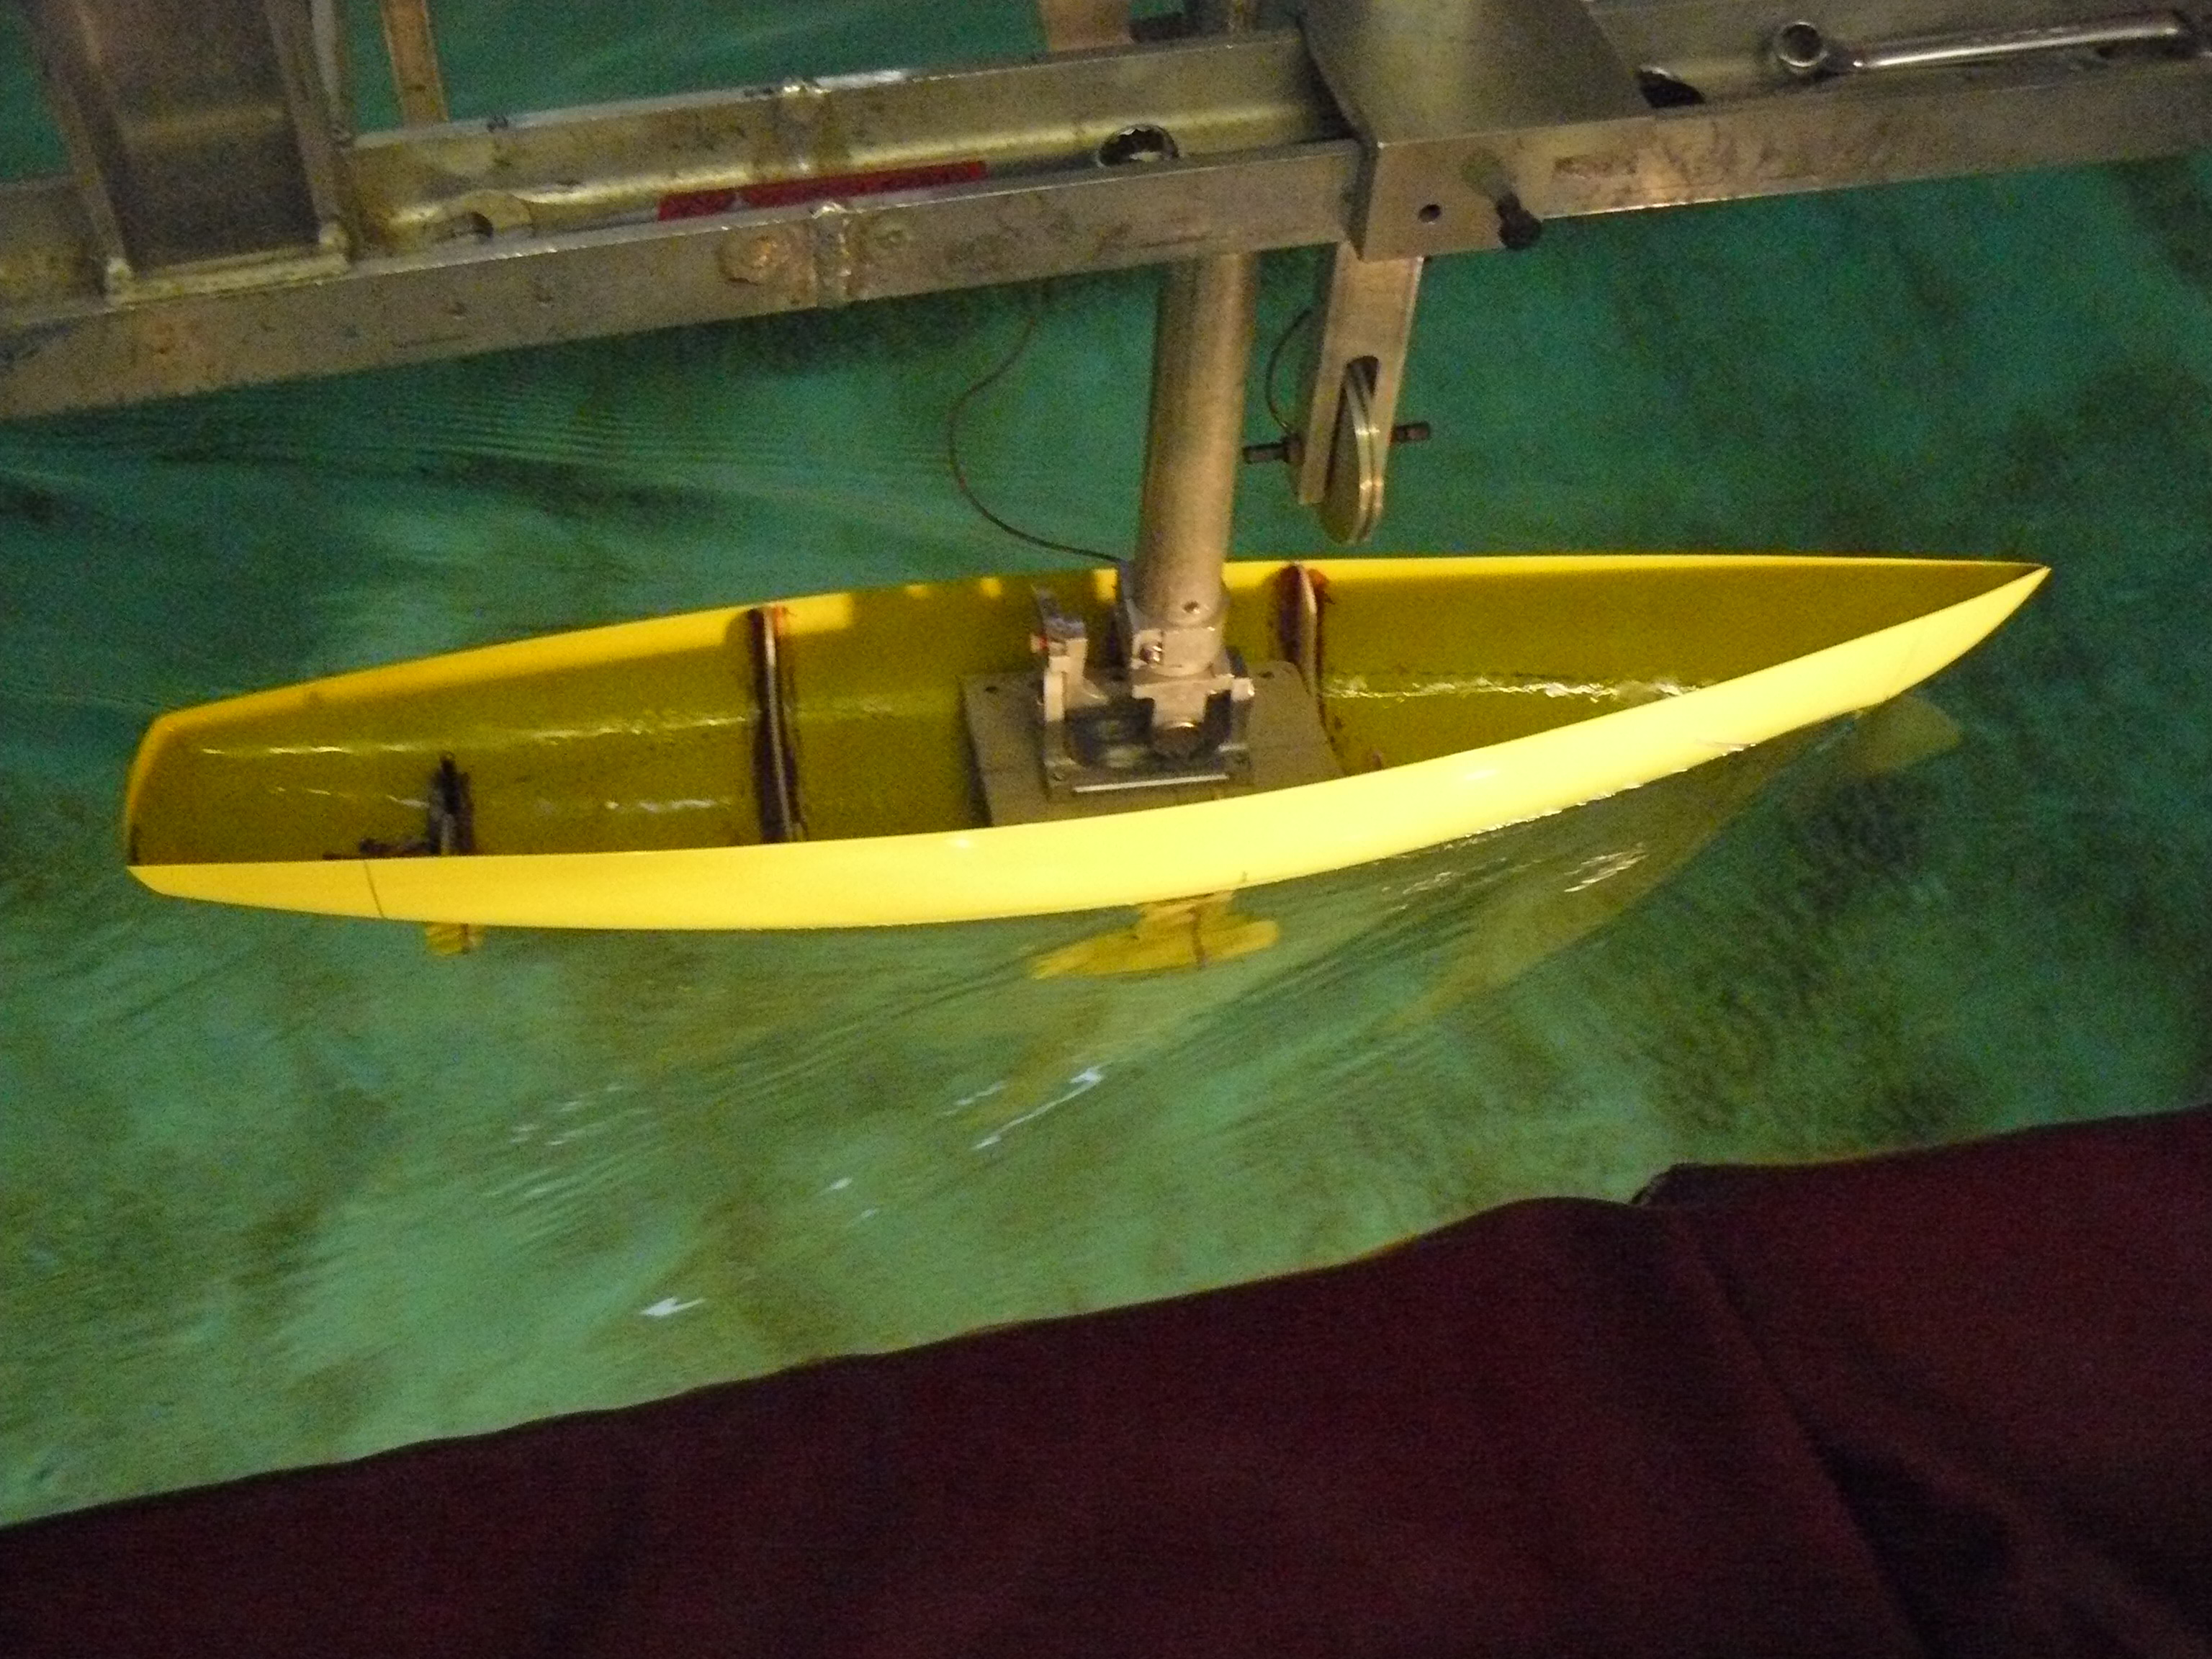
\includegraphics[height=3.5cm]{figures/carene} \qquad 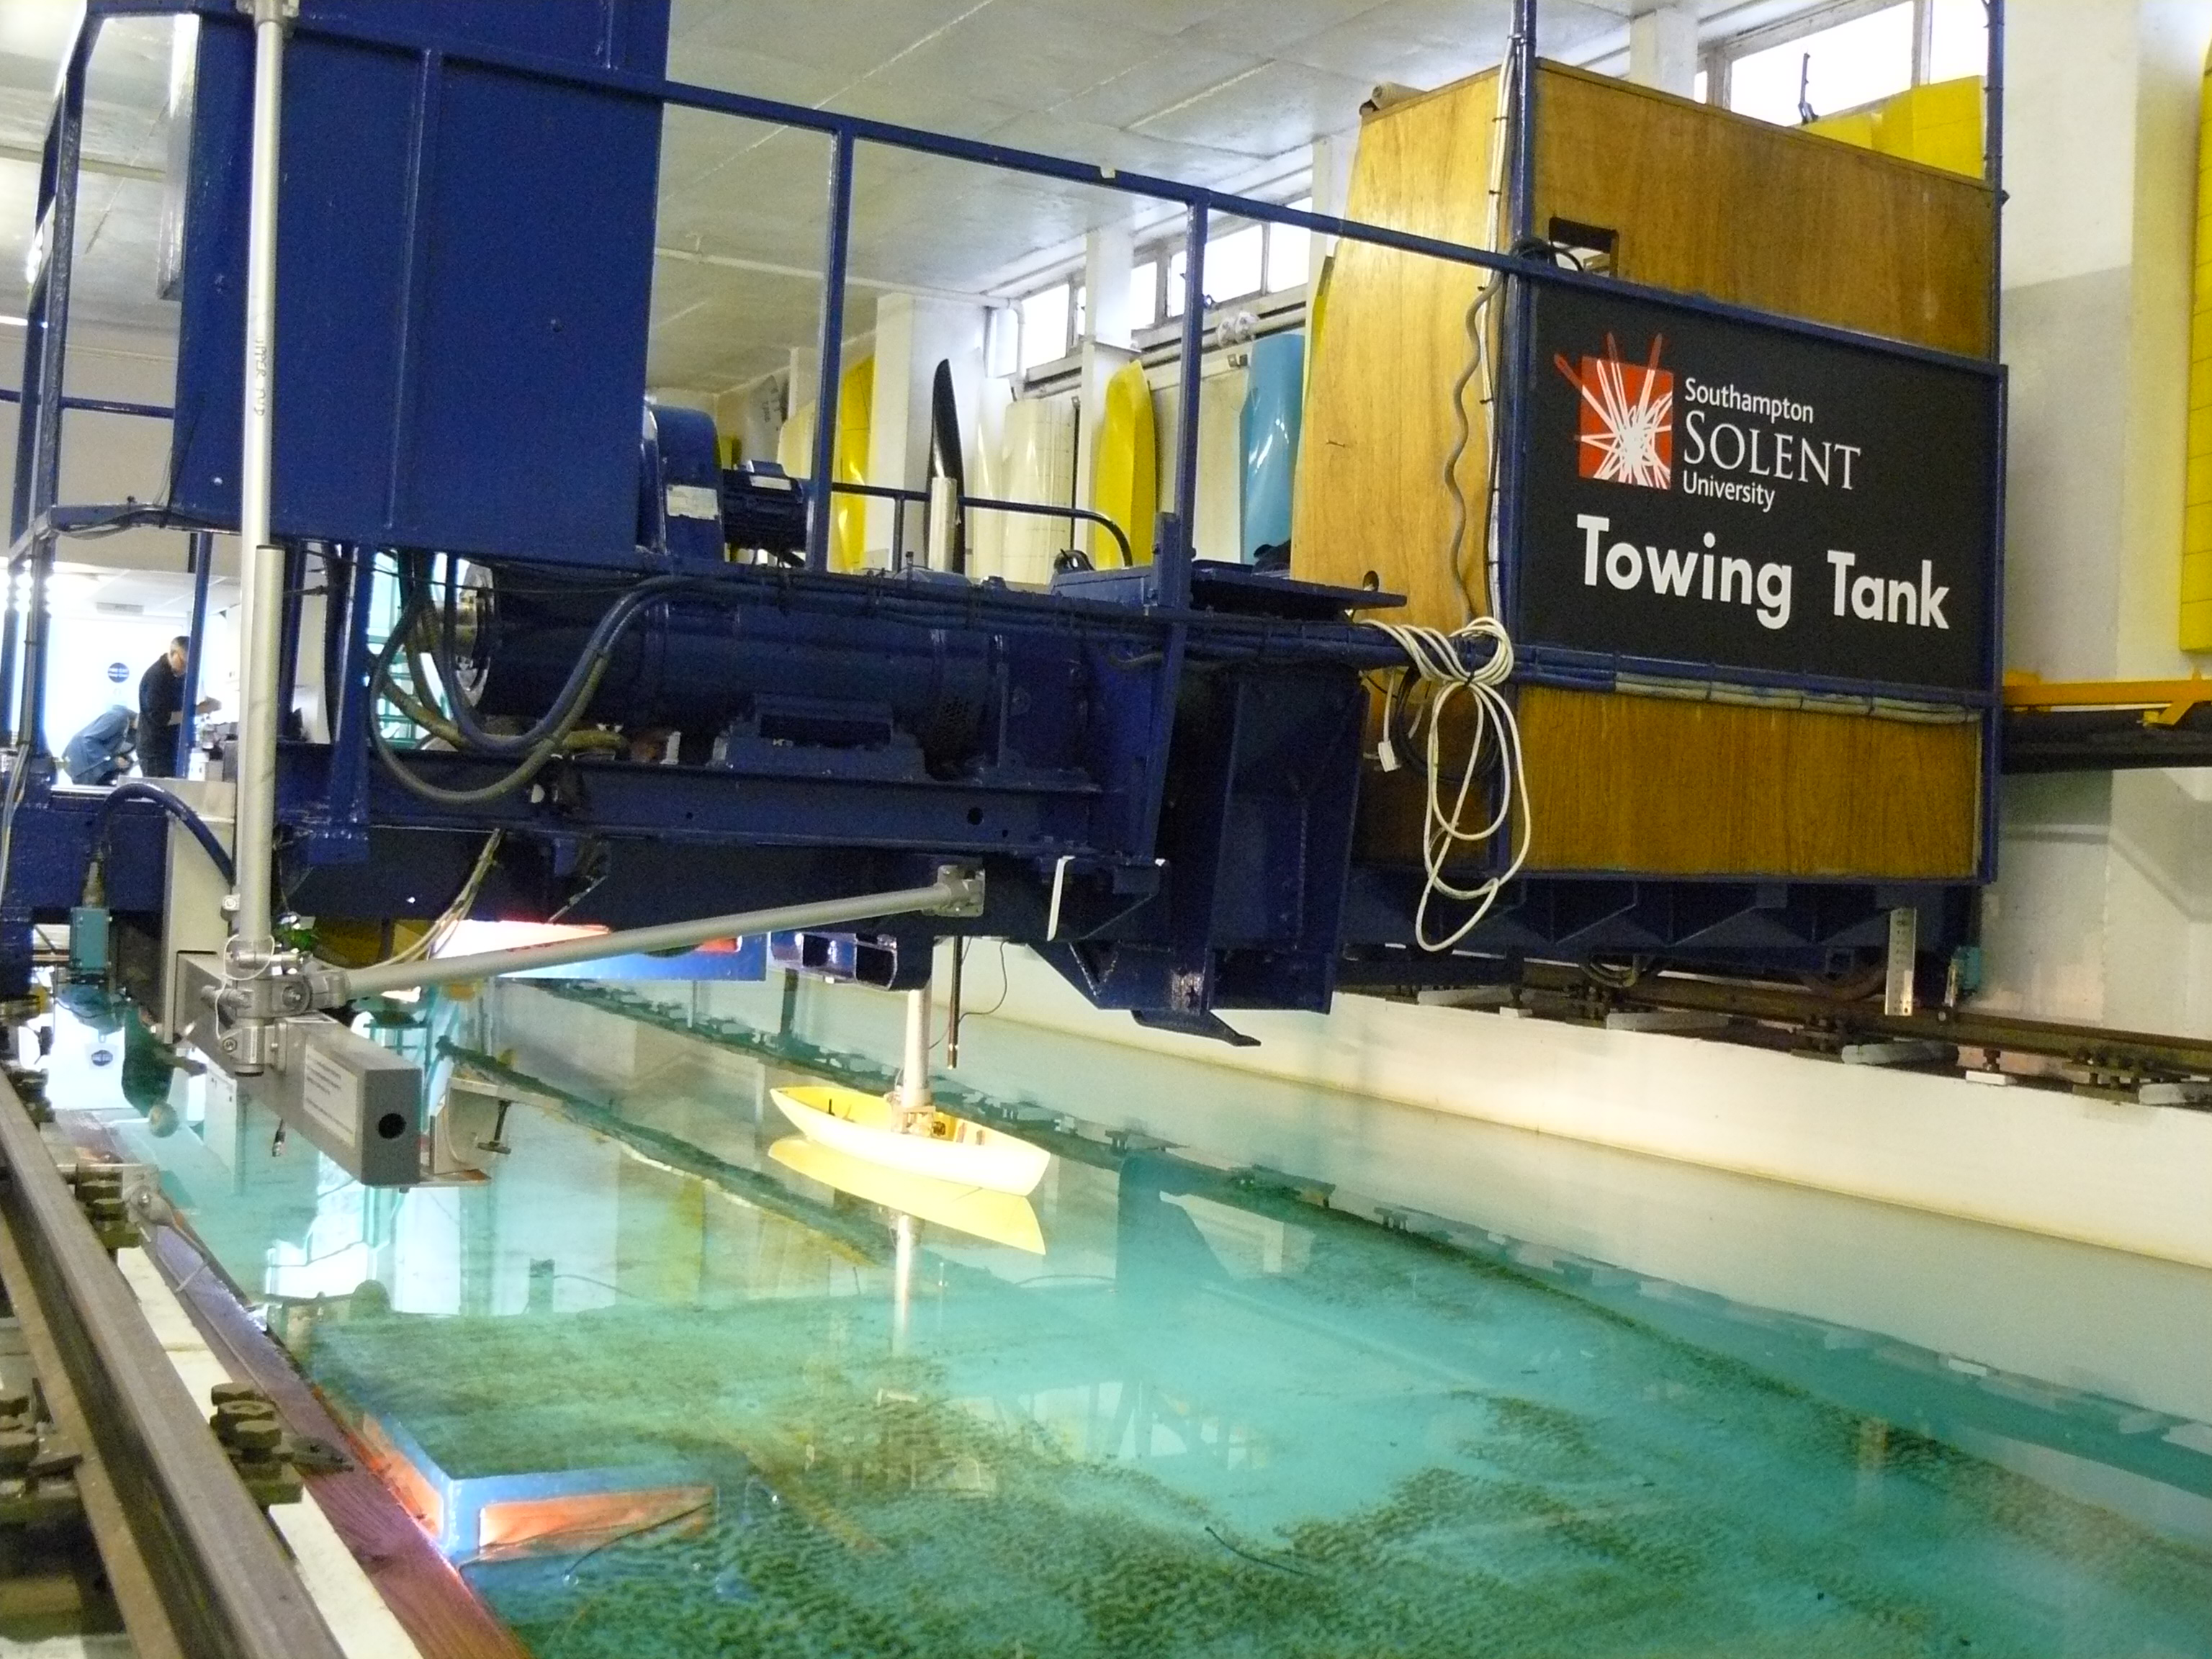
\includegraphics[height=3.5cm]{figures/carene2}
\end{center}
Knowing the drag for a given design requires costly experiments
\end{exampleblock}
\end{frame}

%%%%%%%%%%%%%%%%%%%%%%%%%%%%%%%%%%%%%%%%%%%%%%%%%%%%%%
\begin{frame}{}
\begin{exampleblock}{Example: Numerical experiments}
\begin{center}
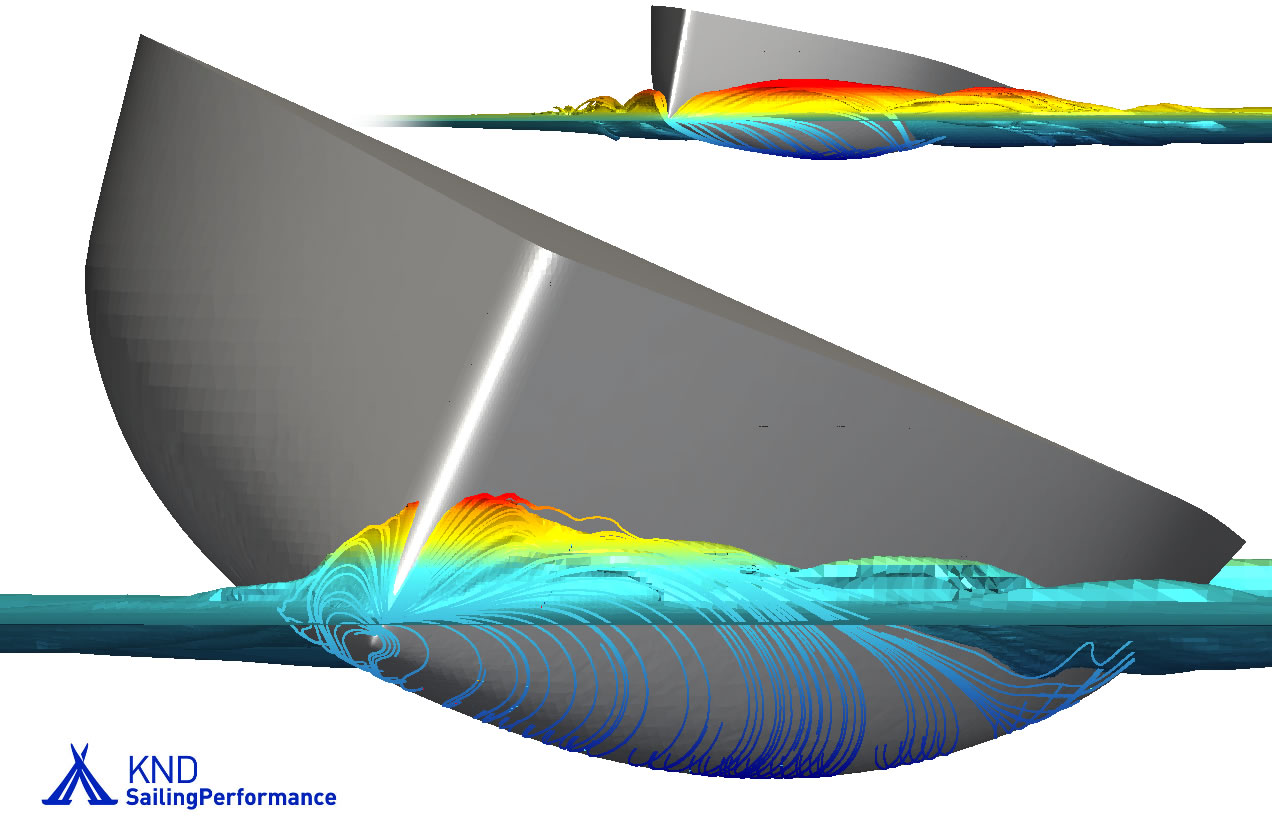
\includegraphics[height=2.8cm]{figures/waterflow} \qquad 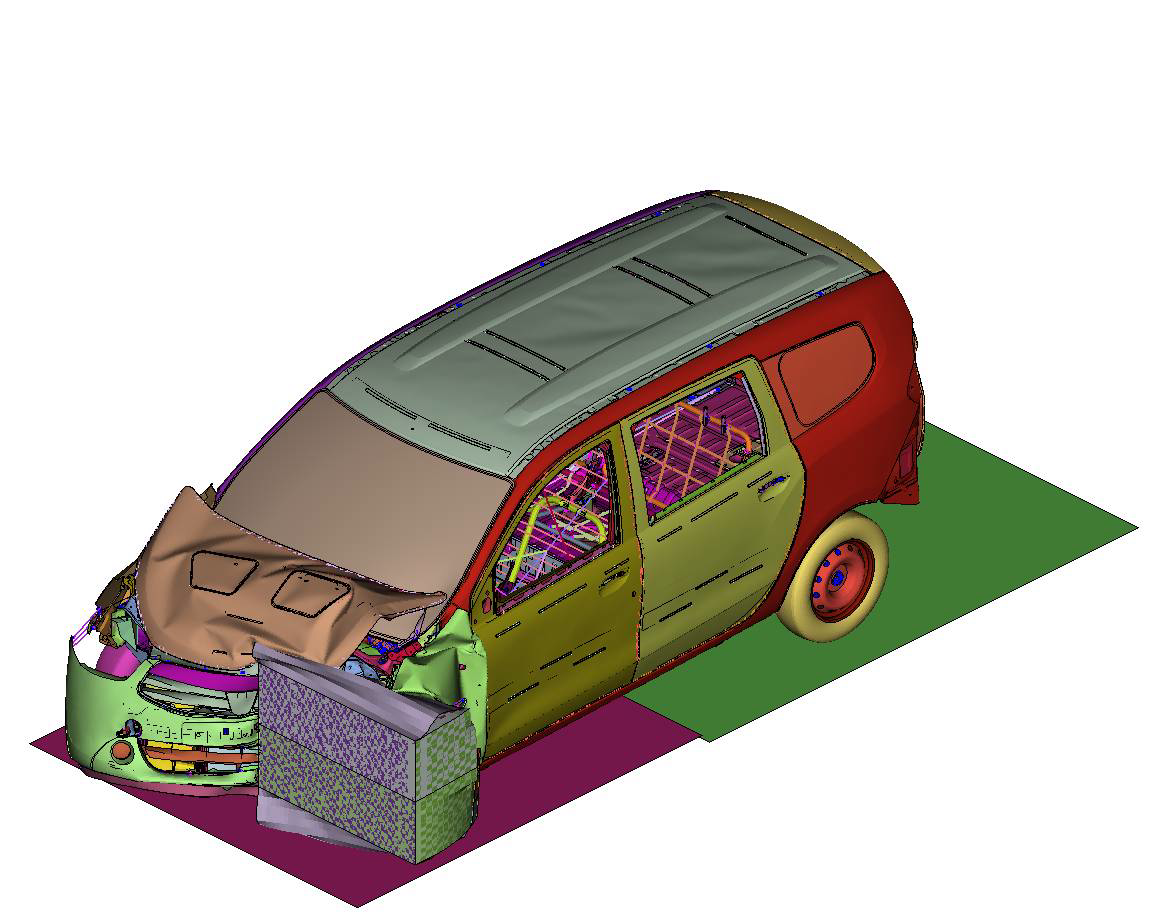
\includegraphics[height=4.2cm]{figures/image15}
\end{center}
Numerical experiments are less expensive but can be very time consuming!
\end{exampleblock}
\end{frame}

%%%%%%%%%%%%%%%%%%%%%%%%%%%%%%%%%%%%%%%%%%%%%%%%%%%%%%
\begin{frame}{}
In all these cases, the variable of interest can be seen as a function of the input parameters
$$ y = f(x). $$
where $f$ is a \textbf{costly to evaluate function}. \\
\vspace{5mm}
In the following, we will assume that 
\begin{itemize}
	\item $x \in \mathds{R}^d$: There are many input parameters
	\item $y \in \mathds{R}$: The output is a scalar.
\end{itemize}
\end{frame}

%%%%%%%%%%%%%%%%%%%%%%%%%%%%%%%%%%%%%%%%%%%%%%%%%%%%%%
\begin{frame}{}
The fact that $f$ is \textbf{costly to evaluate} changes a lot of things...\\
\vspace{5mm}
\structure{1. Representing the function is not possible...}\\
\vspace{5mm}
\begin{center}
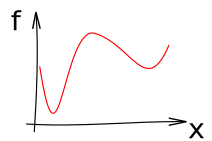
\includegraphics[height=3.2cm]{figures/ink_f} 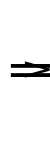
\includegraphics[height=3.2cm]{figures/Rightarrow} 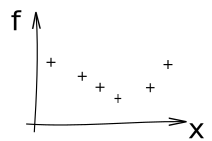
\includegraphics[height=3.2cm]{figures/ink_fX}
\end{center}
\end{frame}

%%%%%%%%%%%%%%%%%%%%%%%%%%%%%%%%%%%%%%%%%%%%%%%%%%%%%%
\begin{frame}{}
The fact that $f$ is \textbf{costly to evaluate} changes a lot of things...\\
\vspace{5mm}
\structure{2. Computing integrals is not possible...}\\
\vspace{5mm}
\begin{center}
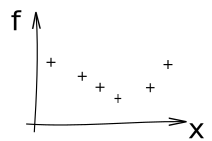
\includegraphics[height=4.5cm]{figures/ink_fX}
\end{center}
What is the mean value of $f$?
\end{frame}

%%%%%%%%%%%%%%%%%%%%%%%%%%%%%%%%%%%%%%%%%%%%%%%%%%%%%%
\begin{frame}{}
The fact that $f$ is \textbf{costly to evaluate} changes a lot of things...\\
\vspace{5mm}
\structure{3. Uncertainty propagation is not possible...}\\
\vspace{5mm}
\begin{center}
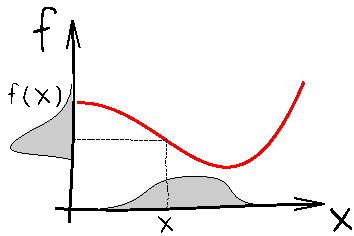
\includegraphics[height=3.2cm]{figures/ink_unprogf} 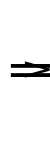
\includegraphics[height=3.2cm]{figures/Rightarrow} 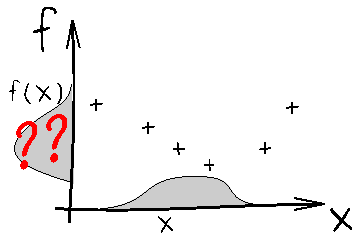
\includegraphics[height=3.2cm]{figures/ink_unprogfX}
\end{center}
\end{frame}

%%%%%%%%%%%%%%%%%%%%%%%%%%%%%%%%%%%%%%%%%%%%%%%%%%%%%%
\begin{frame}{}
The fact that $f$ is \textbf{costly to evaluate} changes a lot of things...\\
\vspace{5mm}
\structure{4. Sensitivity analysis is not possible...}\\
\vspace{5mm}
\begin{center}
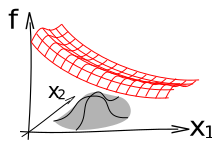
\includegraphics[height=4.5cm]{figures/ink_as}
\end{center}
\end{frame}

%%%%%%%%%%%%%%%%%%%%%%%%%%%%%%%%%%%%%%%%%%%%%%%%%%%%%%
\begin{frame}{}
The fact that $f$ is \textbf{costly to evaluate} changes a lot of things...\\
\vspace{5mm}
\structure{5. Optimisation is also tricky...}\\
\vspace{5mm}
\begin{center}
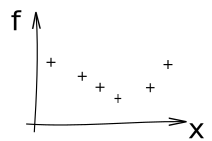
\includegraphics[height=4.5cm]{figures/ink_fX}
\end{center}
\end{frame}

%%%%%%%%%%%%%%%%%%%%%%%%%%%%%%%%%%%%%%%%%%%%%%%%%%%%%%
%%%%%%%%%%%%%%%%%%%%%%%%%%%%%%%%%%%%%%%%%%%%%%%%%%%%%%
\section[Statistical models]{Statistical models}
\subsection{}

%%%%%%%%%%%%%%%%%%%%%%%%%%%%%%%%%%%%%%%%%%%%%%%%%%%%%%
\begin{frame}{}
The principle of statistical modelling is to use the data to build a mathematical approximation of the function. 
\begin{center}
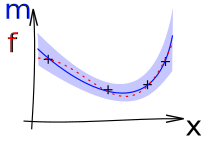
\includegraphics[height=4.5cm]{figures/ink_m}
\end{center}
The model can then be used to answer all previous questions
\end{frame}

%%%%%%%%%%%%%%%%%%%%%%%%%%%%%%%%%%%%%%%%%%%%%%%%%%%%%%
\begin{frame}{}
Of course, there is a difference between $f$ and $m$...
\begin{center}
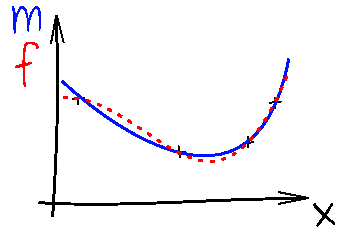
\includegraphics[height=5cm]{figures/ink_mf}
\end{center}
\end{frame}

%%%%%%%%%%%%%%%%%%%%%%%%%%%%%%%%%%%%%%%%%%%%%%%%%%%%%%
\begin{frame}{}
Why \textbf{statistical models}? \\We want to be able to quantify the model error:
\begin{center}
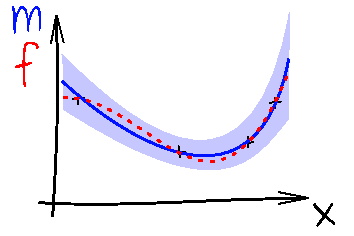
\includegraphics[height=5cm]{figures/ink_mconfint}
\end{center}
The confidence intervals can be used to obtain a \textbf{measure of uncertainty on the value of interest}.
\end{frame}

%%%%%%%%%%%%%%%%%%%%%%%%%%%%%%%%%%%%%%%%%%%%%%%%%%%%%%
\begin{frame}{}
In the sequel, we will use the following notations : 
\begin{itemize}
	\item The set of observation points will be represented by a $n \times d$ matrix $X=(X_1, ..., X_n)^t$
	\item The vector of observations will be denoted by $F$ : $F_i=f(X_i)$ (or $F=f(X)$).
\end{itemize}
    Before discussing statistical models (tomorrow), we will talk about \textbf{design of experiments}
\begin{itemize}
    \item[] If you have a budget of $n$ function calls, which points of the input space should be evaluated?
\end{itemize}
\end{frame}

%%%%%%%%%%%%%%%%%%%%%%%%%%%%%%%%%%%%%%%%%%%%%%%%%%%%%%
%%%%%%%%%%%%%%%%%%%%%%%%%%%%%%%%%%%%%%%%%%%%%%%%%%%%%%
\section[DoE]{Design of Experiments}
\subsection{}

%%%%%%%%%%%%%%%%%%%%%%%%%%%%%%%%%%%%%%%%%%%%%%%%%%%%%%
\begin{frame}{}
Intuition is often misleading in high-dimension:
\begin{exampleblock}{Examples 1/2}
\begin{itemize}
	\item Points in the unit cube can be far away\\ \qquad $\rightarrow$ the diagonal of the unit cube is of length $\sqrt{d}$
	\item All the volume is near the domain boundaries \\ \qquad $\rightarrow$ let us consider a hypercube of size 0.9 included in the the unit cube:\vspace{5mm}
	\begin{center}
\includegraphics[height=4cm]{figures/latexdraw/volumedim} \quad
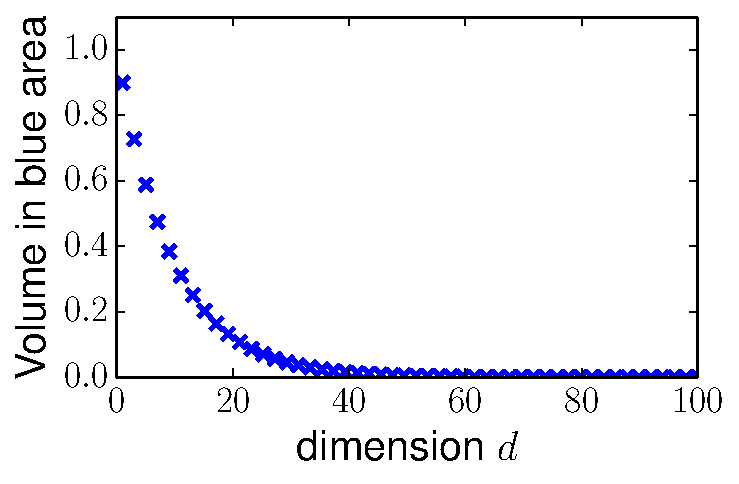
\includegraphics[height=3.5cm]{figures/python/spf_volume}
\end{center}
\end{itemize}
\end{exampleblock}
\end{frame}

%%%%%%%%%%%%%%%%%%%%%%%%%%%%%%%%%%%%%%%%%%%%%%%%%%%%%%
\begin{frame}{}
Intuition is often misleading in high-dimension:
\begin{exampleblock}{Examples 2/2}
\begin{itemize}
	\item The number of vertices of an hypercube increases faster than we usually think
\end{itemize}
\begin{columns}[c]
\column{5.5cm}
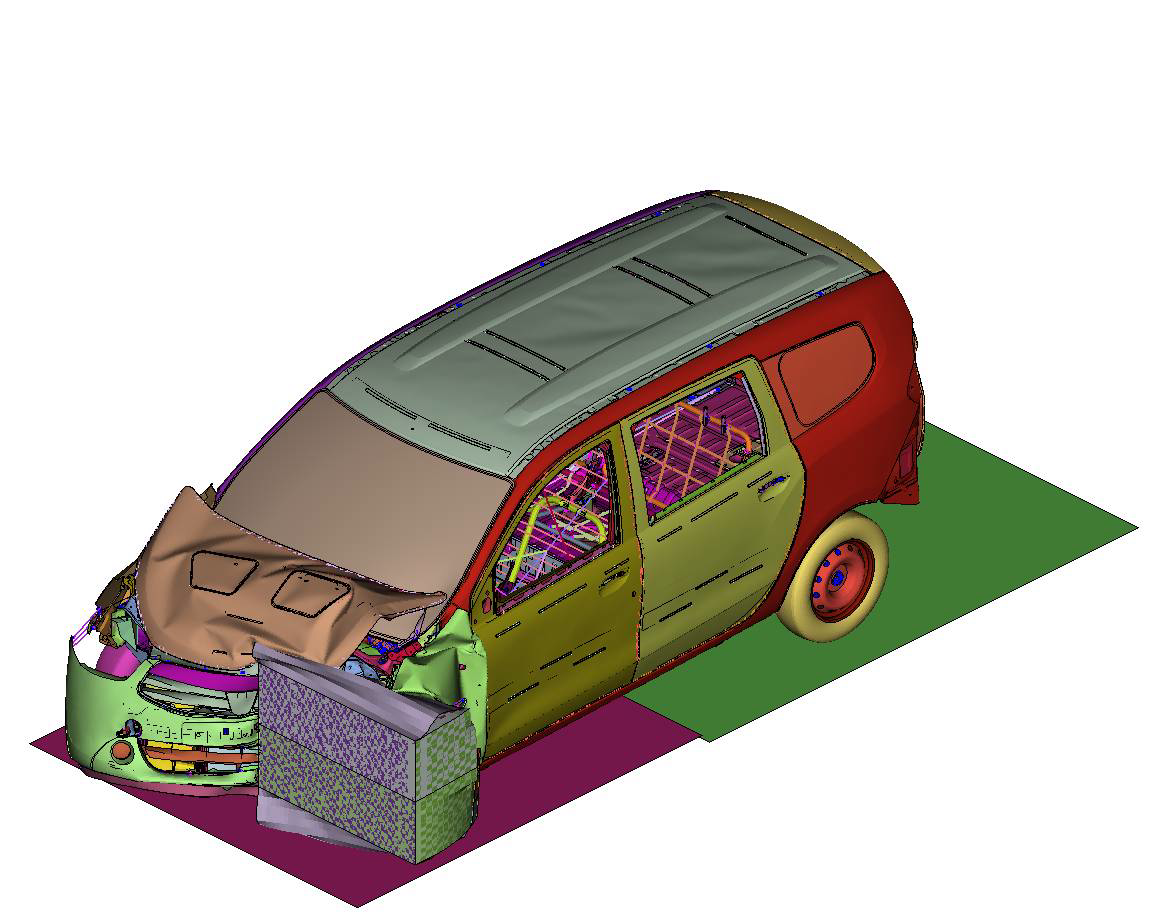
\includegraphics[height=4.5cm]{figures/image15}
\column{5cm}
Testing all combinations of min and max input values for the 50 parameters would require... \pause \\

\textbf{3000 times the age of the universe}!\\
($d=50$ $\rightarrow$ $2^d \approx 1.e15$)
\end{columns}
\end{exampleblock}
\end{frame}

%%%%%%%%%%%%%%%%%%%%%%%%%%%%%%%%%%%%%%%%%%%%%%%%%%%%%%
\begin{frame}{One at a time design}
An intuitive way to check the influence of various variable is to make them change one at the time.
\begin{itemize}
	\item All variables are fixed at a reference value (0 for example)
	\item One variable is changed at a time to see if there is an influence
\end{itemize}
\vspace{5mm}
\begin{example}
\begin{columns}[c]
\column{5cm}
\begin{center}
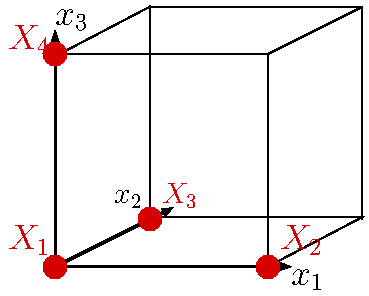
\includegraphics[width=4cm]{figures/latexdraw/1atatime}
\end{center}
\column{5cm}
\begin{center}
  \begin{tabular}{|c|ccc|}
  \hline
  point & $x_1$ & $x_2$ & $x_3$ \\ \hline
  $X_1$ & 0 & 0 & 0 \\
  $X_2$ & 1 & 0 & 0 \\
  $X_3$ & 0 & 1 & 0 \\
  $X_4$ & 0 & 0 & 1 \\ \hline
  \end{tabular}
\end{center}
\end{columns}
\end{example}
\end{frame}

%%%%%%%%%%%%%%%%%%%%%%%%%%%%%%%%%%%%%%%%%%%%%%%%%%%%%%
\begin{frame}{}
\textbf{pros and cons of this kind of design}:
\begin{itemize}
  \item[+] require only $d+1$ observations
  \item[+] are easy to interpret
  \item[] \vspace{-4mm}
  \item[$-$] they can only see linear effects:
  \begin{center}
  $m(x)=\beta_0 + \beta_1 x_1 + \beta_2 x_2 + \beta_3 x_3$
  \end{center}
  \item[$-$] they do not cover the space
\end{itemize}
\vspace{5mm}
\begin{exampleblock}{Exercise}
How can this kind of design be adapted to estimate quadratic effect?
\end{exampleblock}
\end{frame}

%%%%%%%%%%%%%%%%%%%%%%%%%%%%%%%%%%%%%%%%%%%%%%%%%%%%%%
\begin{frame}{}
\begin{exampleblock}{Solution}
Quadratic effects can be estimated with either
\begin{center}
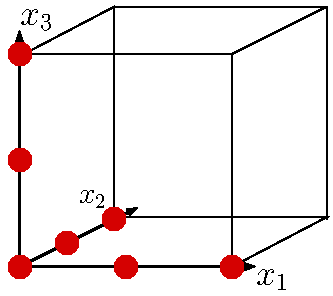
\includegraphics[width=4.5cm]{figures/latexdraw/1atatime1} \hspace{10mm}
\includegraphics[width=4.5cm]{figures/latexdraw/1atatime2}
\end{center}
we sometime talk about ``star shaped'' design.
\end{exampleblock}
\end{frame}

%%%%%%%%%%%%%%%%%%%%%%%%%%%%%%%%%%%%%%%%%%%%%%%%%%%%%%
\begin{frame}{Factorial designs}
The principle of factorial design is to consider all combinations for $x_i \in \{0,1\}$:
\vspace{5mm}
\begin{columns}[c]
\column{4cm}
\begin{center}
\includegraphics[width=4cm]{figures/latexdraw/factorial}
\end{center}
\column{6cm}
\begin{itemize}
	\item[\textbf{pros}] They allow to get all interaction terms:
\end{itemize}
	$$\beta_0 + \sum_k \beta_k x_k + \sum_{j,k} \beta_{j,k} x_j x_k  + \beta_{1,2,3} x_1 x_2 x_3$$
\begin{itemize}
	\item[\textbf{cons}] The number of evaluation is unrealistic when $d$ is large
\end{itemize}
\end{columns}
\end{frame}

%%%%%%%%%%%%%%%%%%%%%%%%%%%%%%%%%%%%%%%%%%%%%%%%%%%%%%
\begin{frame}{Factorial designs}
It is also possible to build factorial designs with $k$ levels:
\begin{center}
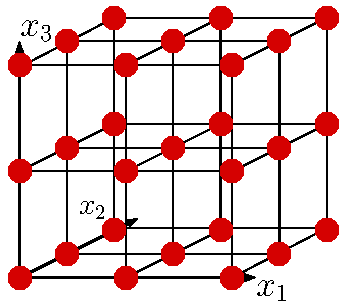
\includegraphics[width=5cm]{figures/latexdraw/factorial3levels}
\end{center}
This allows to compute quadratic effects but the number of evaluations $k^d$ is even less realistic...
\end{frame}

%%%%%%%%%%%%%%%%%%%%%%%%%%%%%%%%%%%%%%%%%%%%%%%%%%%%%%
\begin{frame}{}
\textbf{Conclusion on classical designs:}\\
\structure{\textbf{pros:}}\\
\quad Easy to use\\
\quad adapted to continuous or discrete variables\\
\quad Can be combined (star + factorial for example)\\
\quad Well suited (often optimal) for linear regression\\
\vspace{5mm}
\structure{\textbf{cons:}}\\
\quad Number of evaluation is not flexible\\
\quad Number of evaluation too large in high dimension\\
\quad Points are on top of each other when projected
\end{frame}

%%%%%%%%%%%%%%%%%%%%%%%%%%%%%%%%%%%%%%%%%%%%%%%%%%%%%%
\begin{frame}{projection issues}
Why don't we want points to be superimposed when projected?\\
If one of the variables has no influence, most observations become redundant...
\begin{center}
\includegraphics[height=4.5cm]{figures/latexdraw/factorialprojection}
\end{center}
From 27 observations, we end up with only 9...
\end{frame}

%%%%%%%%%%%%%%%%%%%%%%%%%%%%%%%%%%%%%%%%%%%%%%%%%%%%%%
%%%%%%%%%%%%%%%%%%%%%%%%%%%%%%%%%%%%%%%%%%%%%%%%%%%%%%
\section{Space filling DoE}
\subsection{}


%%%%%%%%%%%%%%%%%%%%%%%%%%%%%%%%%%%%%%%%%%%%%%%%%%%%%%
\begin{frame}{}
We will now focus on designs of experiments that:
\begin{itemize}
	\item are not model oriented
	\item give information about every domain of the input space
	\item have good projection on subspaces
	\item have a flexible number of points
\end{itemize}
\end{frame}

%%%%%%%%%%%%%%%%%%%%%%%%%%%%%%%%%%%%%%%%%%%%%%%%%%%%%%
\begin{frame}{}
How can we evaluate if a set of points fills the space?\\ \vspace{5mm}
\textbf{Option 1.} Compute distances between points\\
\begin{itemize}
	\item[maximin] the minimum distance between two points of the design should be large:
	$$\text{Optimisation problem is: \quad} \max_{X_1,\dots,X_n} [ \min_{i \neq j} dist(X_i,X_j) ]$$
	\item[minimax] the maximum distance between any point of the space and closest design point should be small:
	$$\text{Optimisation problem is: \quad} \min_{X_1,\dots,X_n} (\max_{x \in D} [ \min_i dist(x,X_i) ])$$
\end{itemize}
The second criterion is much more difficult to optimise
\end{frame}

%%%%%%%%%%%%%%%%%%%%%%%%%%%%%%%%%%%%%%%%%%%%%%%%%%%%%%
\begin{frame}{}
These criteria can be illustrated on a simple 2-dimensional example
\begin{center}
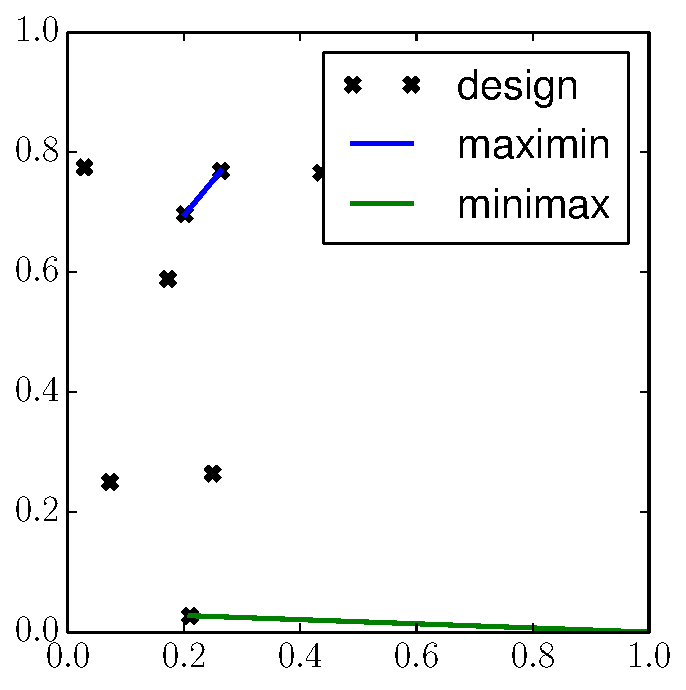
\includegraphics[height=6.5cm]{figures/python/spf_minimaxmaximin}
\end{center}
\end{frame}

%%%%%%%%%%%%%%%%%%%%%%%%%%%%%%%%%%%%%%%%%%%%%%%%%%%%%%
\begin{frame}{}
How can we evaluate if a set of points fills the space?\\ \vspace{2mm}
\textbf{Option 2.} Compare the distribution with an uniform distribution\\ \vspace{2mm}
\structure{Discrepency} is a measure of non uniformity. It compares the number of points in a hyper-rectangle with the expected number of samples from a uniform distribution
\vspace{-2mm}
\begin{columns}[c]
\column{4cm}
\begin{center}
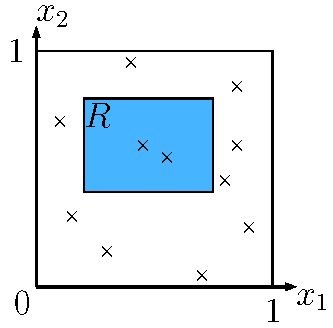
\includegraphics[height=4cm]{figures/latexdraw/discrepency}
\end{center}
\column{6cm}
\vspace{1mm}
The probability for a uniform variable to be in $R$ is 0.22 and we observe an empirical probability of $2/11$. The discrepancy (w.r.t. $R$) is then:
$$D_R = |0.22-2/11| = 0.038$$
\end{columns}
\vspace{2mm}
Discrepency is defined as the sup of the distance between the empirical and analytical cdf.
\end{frame}

%%%%%%%%%%%%%%%%%%%%%%%%%%%%%%%%%%%%%%%%%%%%%%%%%%%%%%
\begin{frame}{}
Discrepency is often computed by:
\begin{itemize}
 	\item fixing one of the hyper-rectangle summit at the origin
 	\item centering the hyper-rectangle
 \end{itemize}
\begin{center}
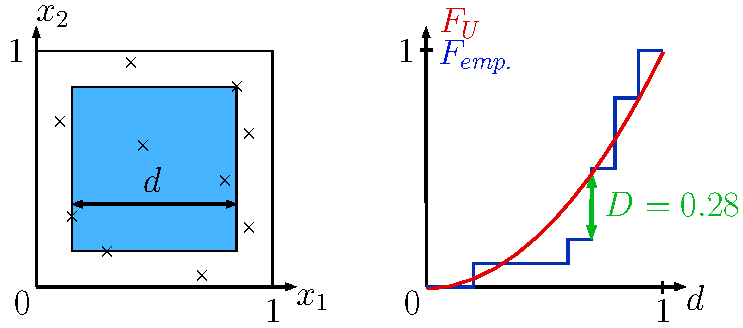
\includegraphics[height=4.5cm]{figures/latexdraw/discrepency3}
\end{center}
The maximum is located where the rectangle is tangent to points\\
$\rightarrow$ The optimisation is over a finite space
\end{frame}

%%%%%%%%%%%%%%%%%%%%%%%%%%%%%%%%%%%%%%%%%%%%%%%%%%%%%%
\begin{frame}{}
We will now give an overview on three types of space filling designs:
\begin{itemize}
	\item Latin hypercubes
	\item low discrepancy sequences
	\item centroidal Voronoi tesselations
\end{itemize}
\end{frame}

%%%%%%%%%%%%%%%%%%%%%%%%%%%%%%%%%%%%%%%%%%%%%%%%%%%%%%
\begin{frame}{Latin hypercubes}
\textbf{Latin hypercubes} are designs where the domain is sliced in $n^d$ blocks and where there is only one point per ``line'' and ``column'':
\begin{center}
\includegraphics[height=5cm]{figures/latexdraw/lhs1}
\end{center}
These designs have good projection properties
\end{frame}


%%%%%%%%%%%%%%%%%%%%%%%%%%%%%%%%%%%%%%%%%%%%%%%%%%%%%%
\begin{frame}{}
A well known example of LHS in 2D is... Sudoku
\vspace{5mm}
\begin{center}
\includegraphics[height=5cm]{figures/sudoku}
\end{center}
\end{frame}

%%%%%%%%%%%%%%%%%%%%%%%%%%%%%%%%%%%%%%%%%%%%%%%%%%%%%%
\begin{frame}{}
If we focus on one digit (say $4$), we obtain a LHD:
\vspace{2mm}
\begin{center}
\includegraphics[height=5cm]{figures/latexdraw/sudoku}
\end{center}
Sudoku have more properties that LHD: the generalisation is called \textbf{orthogonal array}.
\end{frame}

%%%%%%%%%%%%%%%%%%%%%%%%%%%%%%%%%%%%%%%%%%%%%%%%%%%%%%
\begin{frame}{}
Latin hypercubes do not necessarily cover the space very well...
\begin{center}
\includegraphics[height=4.5cm]{figures/latexdraw/lhs2}
\end{center}
They have to be combined with a criterion such as maximin.
\end{frame}

%%%%%%%%%%%%%%%%%%%%%%%%%%%%%%%%%%%%%%%%%%%%%%%%%%%%%%
\begin{frame}{}
\begin{exampleblock}{Exercise}
\begin{itemize}
	\item Generate a 5 points LHD in dimension 3.
	\item How would you program a function \texttt{LHD(n,d)}?
	\item How would you optimize a LHD to ensure it fills the space properly?
\end{itemize}
\end{exampleblock}
\end{frame}

%%%%%%%%%%%%%%%%%%%%%%%%%%%%%%%%%%%%%%%%%%%%%%%%%%%%%%
\begin{frame}{}
\begin{exampleblock}{Solution}
The coordinates of two points can be exchanged:\\
\vspace{4mm}
\begin{center}
\includegraphics[height=4.5cm]{figures/latexdraw/lhs3}
\end{center}
\end{exampleblock}
\end{frame}

%%%%%%%%%%%%%%%%%%%%%%%%%%%%%%%%%%%%%%%%%%%%%%%%%%%%%%
\begin{frame}{}
LHD optimization with simulated annealing:\\
\vspace{4mm}
\textbf{Morris and Mitchell Algorithm}\\
\vspace{2mm}
\begin{itemize}
	\item[1] Generate LHD
	\item[2] find ``bad'' points according to maximin
	\item[3] choose randomly a column of this critical point and exchange it with an randomly selected other point
	\item[4] \qquad if the criteria is improved, the modification is accepted
	\item[5] \qquad otherwise, it is accepted with a probability of $$\exp \left(\frac{maximin_{new}-maximin_{old}}{T}\right)$$
	\end{itemize}
\end{frame}



%%%%%%%%%%%%%%%%%%%%%%%%%%%%%%%%%%%%%%%%%%%%%%%%%%%%%%
\begin{frame}{Low discrepancy sequences}
\textbf{Low discrepancy sequences} are deterministic sequences that converge toward the uniform distribution.
\begin{itemize}
	\item They cover the space quickly and evenly
	\item They are easy to build
	\item It is easy to add new points
\end{itemize}
\vspace{5mm}
Many low discrepancy sequences can be found in the literature: Halton, Hammerley, Sobol', Faure, van der Corput, ...
\end{frame}

%%%%%%%%%%%%%%%%%%%%%%%%%%%%%%%%%%%%%%%%%%%%%%%%%%%%%%
\begin{frame}{}
\begin{example}[Halton sequence]
	Let $a$ and $b$ be two integers with no common dividers (say 2 and 3). The $x_1$ and $x_2$ coordinates of the Halton sequence are:
	\begin{equation*}
		\begin{split}
			x_1 &= 1/2,\ 1/4,\ 3/4,\ 1/8,\ 5/8,\ 3/8,\ 7/8,\ 1/16,\ 9/16, \dots\\
			x_2 &= 1/3,\ 2/3,\ 1/9,\ 4/9,\ 7/9,\ 2/9,\ 5/9,\ 8/9,\ 1/27, \dots
		\end{split}
	\end{equation*}
\begin{center}
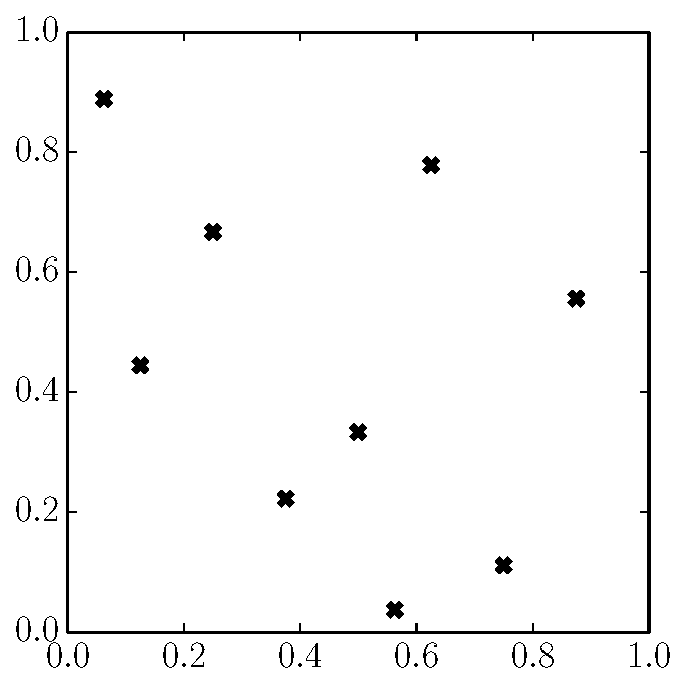
\includegraphics[height=4.5cm]{figures/python/spf_halton}
\end{center}

\end{example}
\end{frame}

%%%%%%%%%%%%%%%%%%%%%%%%%%%%%%%%%%%%%%%%%%%%%%%%%%%%%%
\begin{frame}{}
\begin{example}[Halton sequence]
\begin{center}
  \begin{tabular}{cc}
Halton Sequence & uniform pseudo random \\
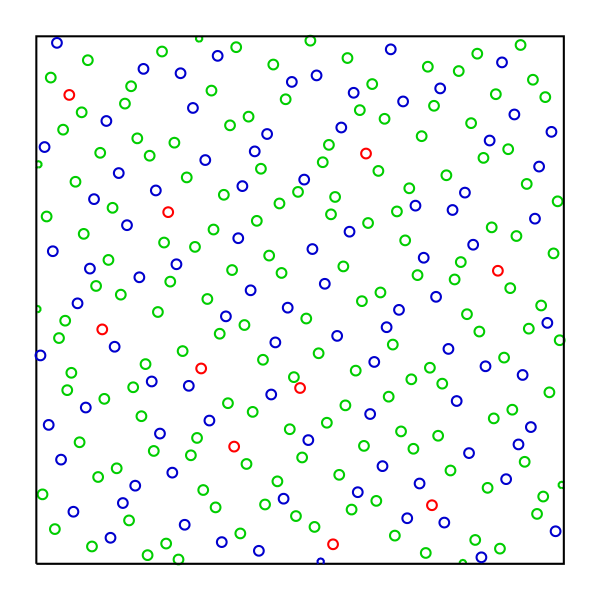
\includegraphics[height=5cm]{figures/Halton} & 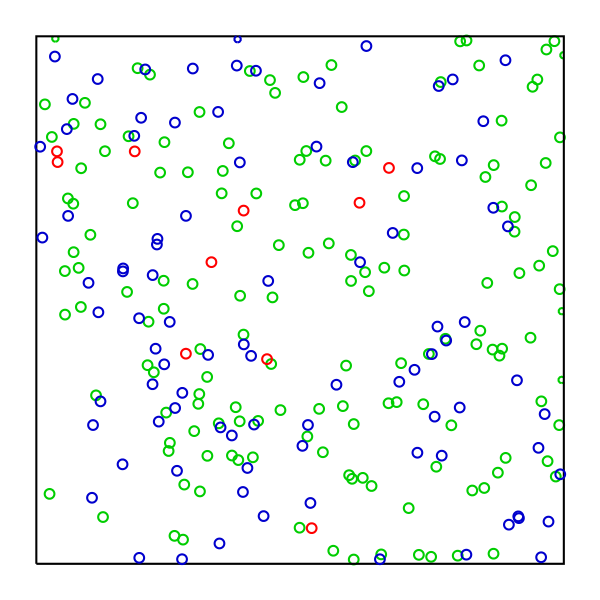
\includegraphics[height=5cm]{figures/random}
  \end{tabular}
 source: wikipedia
\end{center}
\end{example}
\end{frame}

%%%%%%%%%%%%%%%%%%%%%%%%%%%%%%%%%%%%%%%%%%%%%%%%%%%%%%
\begin{frame}{}
Issues with low discrepancy sequences:
\begin{itemize}
	\item[$-$] there can be alignments when projected
	\item[$-$] there can be holes in subspaces
	\item[$-$] points may be aligned (Example: 16 first points in basis (17,18))
\end{itemize}
\end{frame}

%%%%%%%%%%%%%%%%%%%%%%%%%%%%%%%%%%%%%%%%%%%%%%%%%%%%%%
\begin{frame}{Centroidal Voronoi Tesselations}
Given a set of generative points $X$, the \textbf{Voronoi Tesselations} (or Voronoi cells) associated to the point $X_i$ is the region of the space such that $X_i$ is the closest point from the set:
\begin{center}
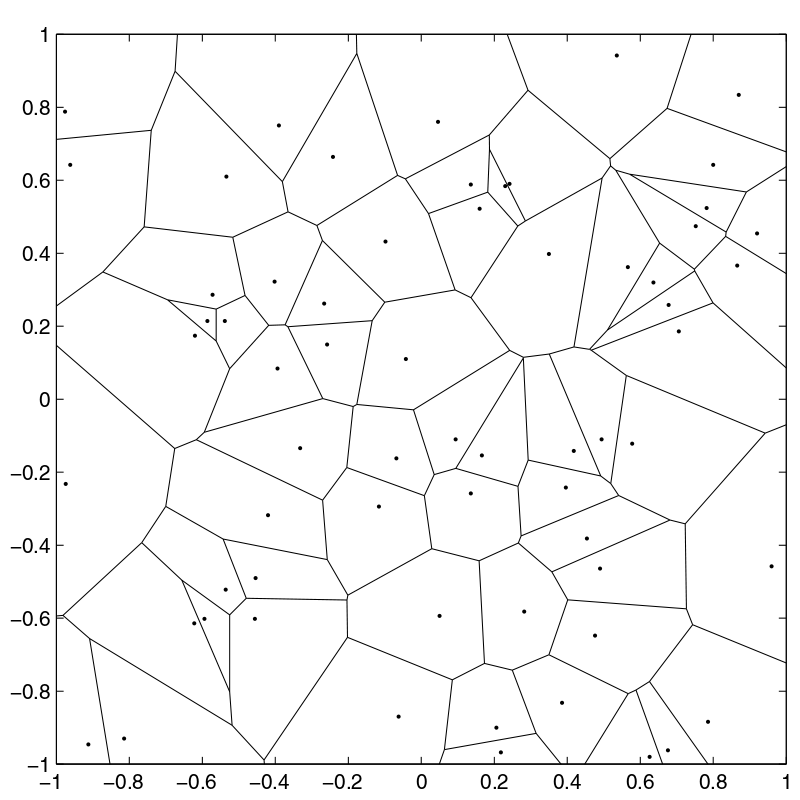
\includegraphics[height=5cm]{figures/VT}
\end{center}
Source: Q. Du et Al., \emph{Centroidal Voronoi Tessellations: Applications and Algorithms}, SIAM Review, 41-4, 1999.
\end{frame}

%%%%%%%%%%%%%%%%%%%%%%%%%%%%%%%%%%%%%%%%%%%%%%%%%%%%%%
\begin{frame}{}
\textbf{Centroidal Voronoi Tesselations (CVT)} is a special case of Voronoi Tesselations where the generative points correspond to the centre of mass of the cells
\begin{center}
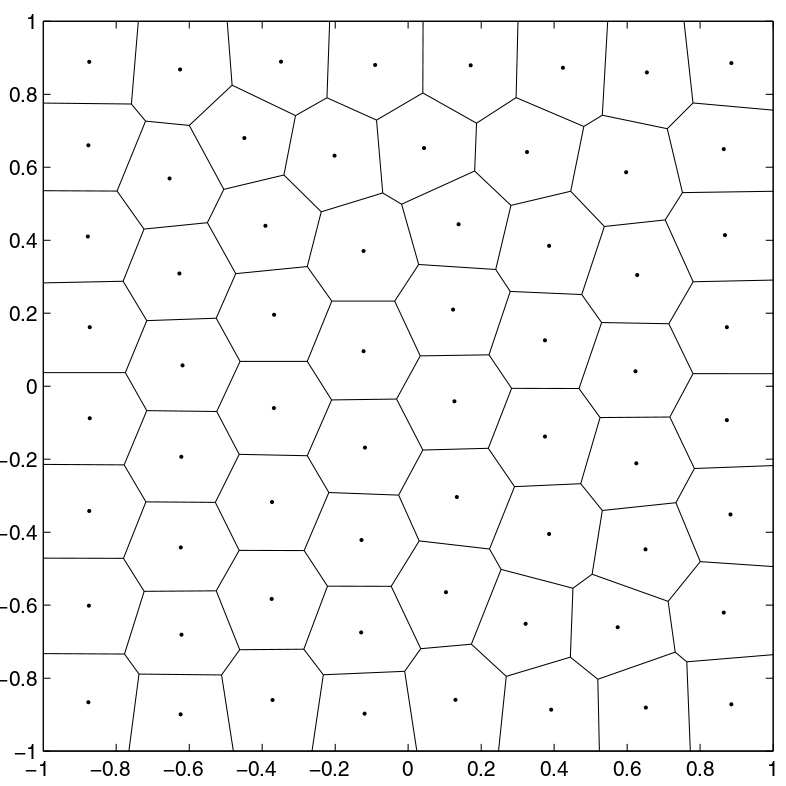
\includegraphics[height=5cm]{figures/CVT}
\end{center}
Source: Q. Du et Al., \emph{Centroidal Voronoi Tessellations: Applications and Algorithms}, SIAM Review, 41-4, 1999.
\end{frame}

%%%%%%%%%%%%%%%%%%%%%%%%%%%%%%%%%%%%%%%%%%%%%%%%%%%%%%
\begin{frame}{}

Properties of CVT:
\begin{itemize}
	\item Each point of the space is close to one generative points
	\item The generative points cover the space
\end{itemize}
$\Rightarrow$ The generative points of CVT can be used as design of experiment.
\end{frame}

%%%%%%%%%%%%%%%%%%%%%%%%%%%%%%%%%%%%%%%%%%%%%%%%%%%%%%
\begin{frame}{Generating CVT }
\textbf{1. Lloyd's Algorithm}
\begin{itemize}
	\item[1] Initialize $X$ as a set of $n$ points
	\item[2] While $i<nb\_iter$
	\item[3] \qquad Compute the Voronoi diagram of $X$
	\item[4] \qquad X = centre of mass of each cell
\end{itemize}
\begin{center}
  \begin{tabular}{cccc}
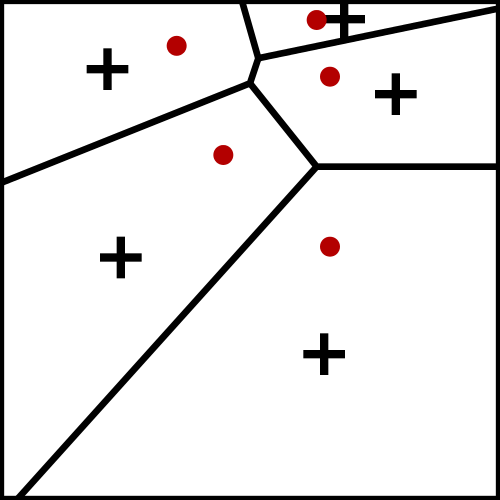
\includegraphics[height=2.4cm]{figures/Lloyds1}&
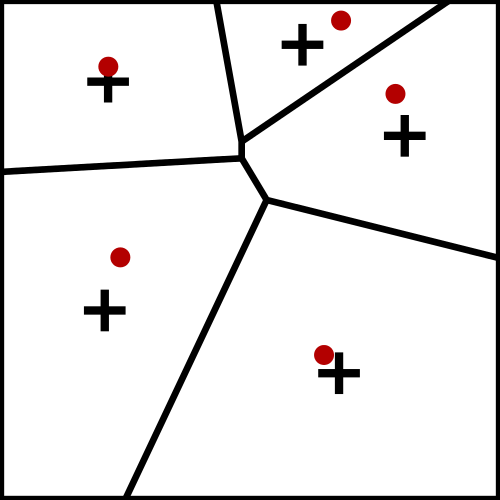
\includegraphics[height=2.4cm]{figures/Lloyds2}&
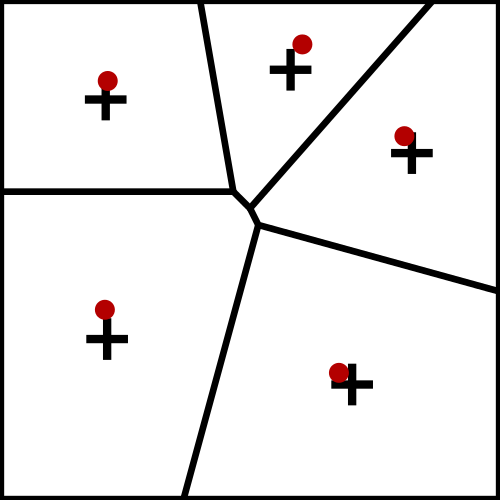
\includegraphics[height=2.4cm]{figures/Lloyds3}&
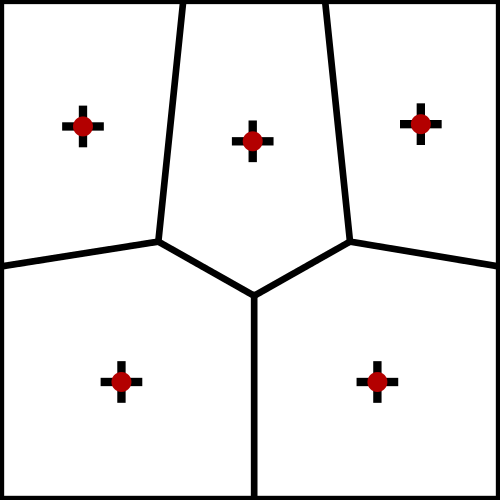
\includegraphics[height=2.4cm]{figures/Lloyds15}\\
iteration 1 & iteration 2 &iteration 3 &iteration 15
  \end{tabular}
\end{center}
source: ``Lloyd's algorithm'' wikipedia page
\end{frame}

%%%%%%%%%%%%%%%%%%%%%%%%%%%%%%%%%%%%%%%%%%%%%%%%%%%%%%
\begin{frame}{Generating CVT }
\textbf{2. k-means}\\
This algorithm is very similar to Lloyd but it uses a large set of points covering the input space instead of the full continuous domain:
\begin{center}
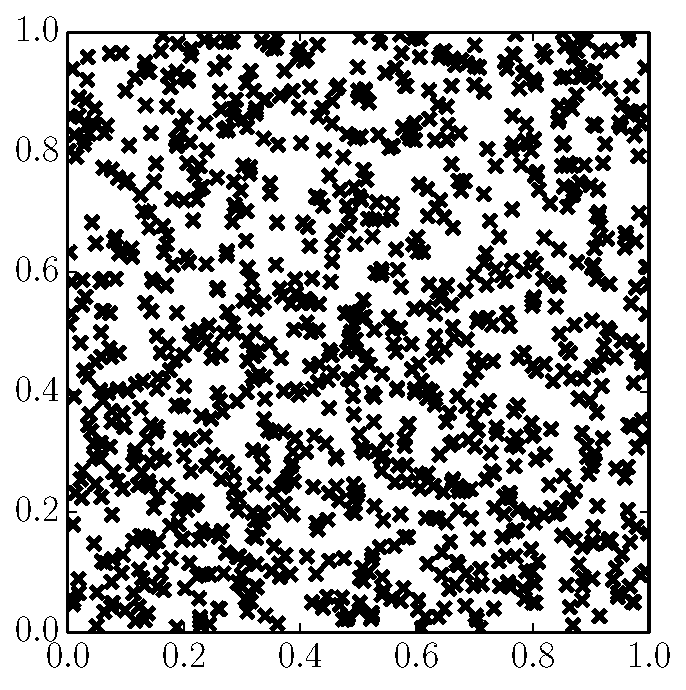
\includegraphics[height=4.5cm]{figures/python/spf_kmeans1}
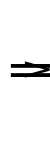
\includegraphics[height=4.5cm]{figures/Rightarrow}
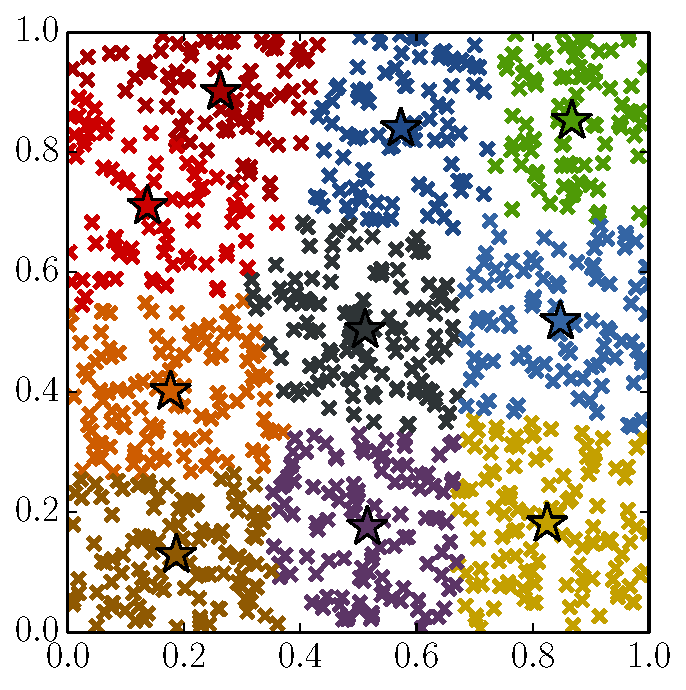
\includegraphics[height=4.5cm]{figures/python/spf_kmeans2}
\end{center}
\end{frame}

%%%%%%%%%%%%%%%%%%%%%%%%%%%%%%%%%%%%%%%%%%%%%%%%%%%%%%
\begin{frame}{Generating CVT }
\textbf{3. McQueen algorithm}\\
\vspace{5mm}
This algorithm is much faster than the previous ones and gives a good approximation
\begin{itemize}
	\item[1] Initialize $X$ as a set of $n$ points
	\item[2] Initialize $k$ as a vector of 1 with length $n$
	\item[3] While $i<nb\_iter$
	\item[4] \qquad generate one random point $z$ in the input space
	\item[5] \qquad find the $X_i$ closest to $z$
	\item[6] \qquad update $X_i = \frac{k_i X_i + z}{k_i+1}$
	\item[7] \qquad $k_i =k_i+1$
\end{itemize}
\end{frame}

%%%%%%%%%%%%%%%%%%%%%%%%%%%%%%%%%%%%%%%%%%%%%%%%%%%%%%
\begin{frame}{Generating CVT }
\textbf{3. McQueen algorithm}\\
We obtain the following design:
\begin{center}
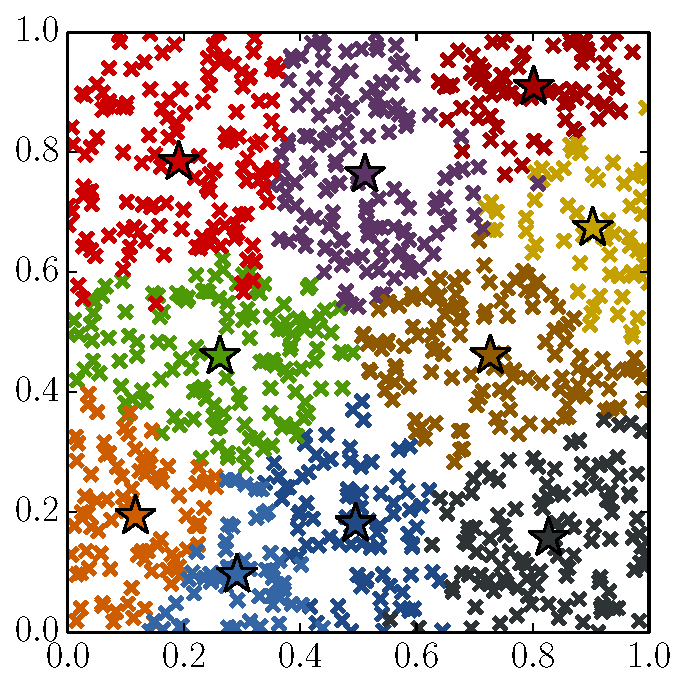
\includegraphics[height=5cm]{figures/python/spf_McQueen}
\end{center}
\end{frame}

%%%%%%%%%%%%%%%%%%%%%%%%%%%%%%%%%%%%%%%%%%%%%%%%%%%%%%
\begin{frame}{}
CVT are not unique:
\begin{center}
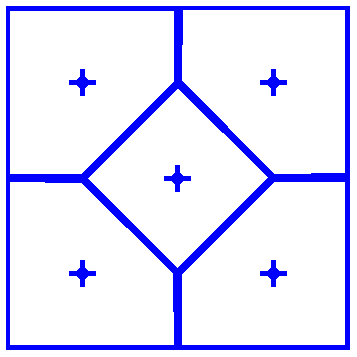
\includegraphics[height=3cm]{figures/CVT1} \qquad
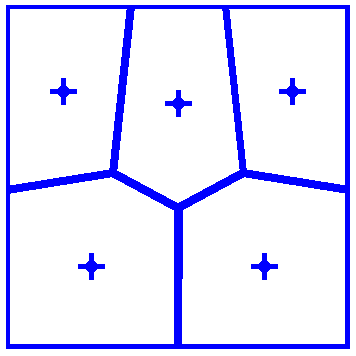
\includegraphics[height=3cm]{figures/CVT2} \qquad
\includegraphics[height=3cm]{figures/CVT3}
\end{center}
 source: wikipedia page ``Centroidal Voronoi Tesselations''
\end{frame}


%%%%%%%%%%%%%%%%%%%%%%%%%%%%%%%%%%%%%%%%%%%%%%%%%%%%%%%%%%%%%%%%%%%%%%%%%%%%%%%
%%%%%%%%%%%%%%%%%%%%%%%%%%%%%%%%%%%%%%%%%%%%%%%%%%%%%%%%%%%%%%%%%%%%%%%%%%%%%%%
%%%%%%%%%%%%%%%%%%%%%%%%%%%%%%%%%%%%%%%%%%%%%%%%%%%%%%%%%%%%%%%%%%%%%%%%%%%%%%%
%%%%%%%%%%%%%%%%%%%%%%%%%%%%%%%%%%%%%%%%%%%%%%%%%%%%%%%%%%%%%%%%%%%%%%%%%%%%%%%
\end{document}













%%%%%%%%%%%%%%%%%%%%%%%%%%%%%%%%%%%%%%%%%%%%%%%%%%%%%%
%%%%%%%%%%%%%%%%%%%%%%%%%%%%%%%%%%%%%%%%%%%%%%%%%%%%%%
%%%%%%%%%%%%%%%%%%%%%%%%%%%%%%%%%%%%%%%%%%%%%%%%%%%%%%

\structure{}

\begin{center}
  \begin{tabular}{|c|cc|}

  \end{tabular}
\end{center}

###
%%%%%%%%%%%%%%%%%%%%%%%%%%%%%%%%%%%%%%%%%%%%%%%%%%%%%%
\begin{frame}{}

\end{frame}

###
\begin{block}{}

\end{block}

###
\begin{center}
\includegraphics[height=5cm]{figures/}
\end{center}

###
\begin{columns}[c]
\column{5cm}

\column{5cm}

\end{columns}
